\clearpage

\section{Práctica 4: Aplicaciones del receptor-emisor infrarrojo}

\subsection{Introducción}

Se tiene un circuito de control que emplea un emisor y recpetor de infrarrojo que controla el encendido y apagado de un rele que controla el estado de un foco de 60W,
el circuito esta sometido a una etapa de alimentación transformeless de 120V, que se convierte a una señal de corriente directa de 12V.

\subsection{Marco teórico}

 \subsubsection{Relevador}

 Se le conoce como relevador a un interruptor que es controlado mediante magnetismo y puede ofrecer o suspender la alimantación de un nodo eléctrico a un sistema.

 \begin{figure}[htb]
     \centering
     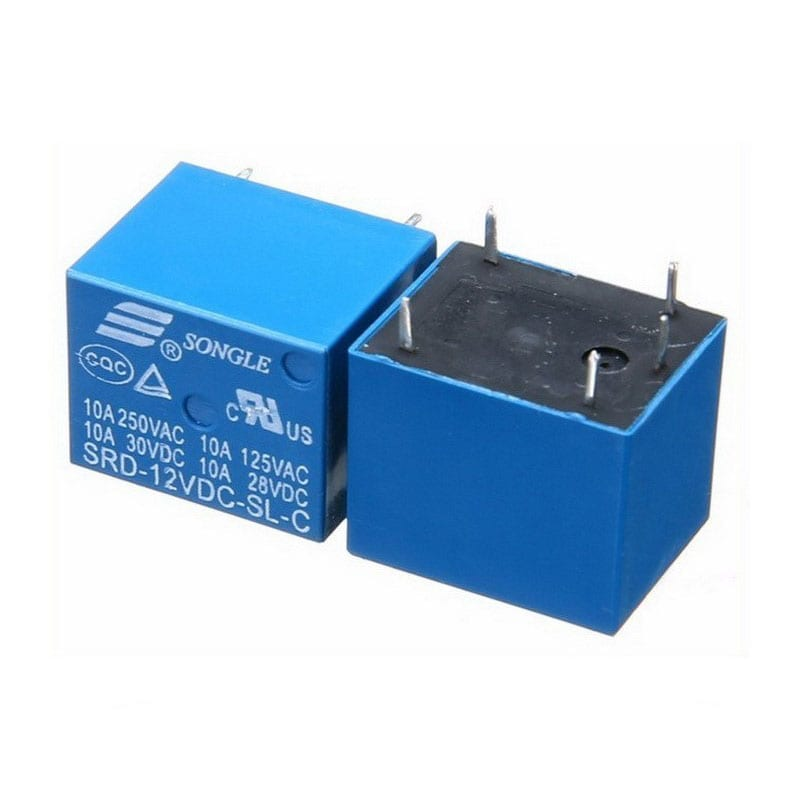
\includegraphics[width=5cm]{media/Rele-12V.jpg}
     \caption{Relevador}
 \end{figure}

\subsubsection{Fototransistor}

Un fototransistor es un tipo de transistor sensible a la luz infrarroja, el cual genera un voltaje cuando le llega la señal de luz, generalmente de un infrarrojo emisor,
y permite accionar una parte del circuito deseado.

\begin{figure}[htb]
    \centering
    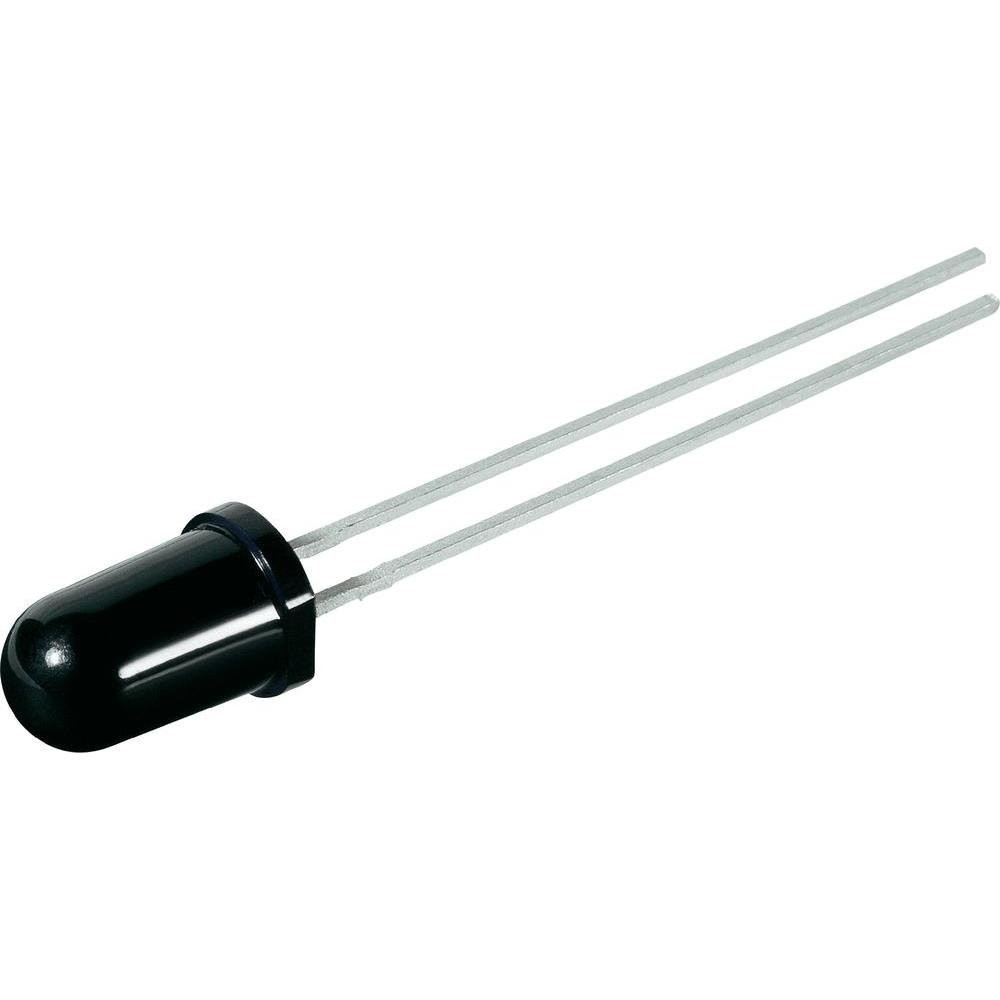
\includegraphics[width=5cm]{media/Fototransistor.jpg}
    \caption{Fototransistor}
\end{figure}

\begin{figure}[htb]
    \centering
    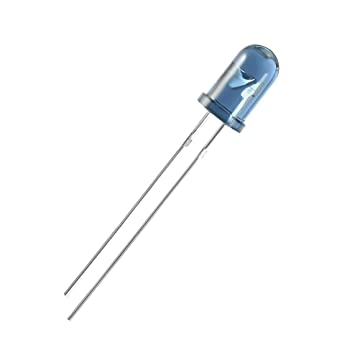
\includegraphics[width=5cm]{media/emisor.jpg}
    \caption{Diodo Emisor de Luz infrarroja}
\end{figure}

\subsubsection{Fuente sin transformador}

Es una fuente a la cual se le conecta a corriente alterna y puede brindar de output un voltaje $V_{out}$ de 12V o 5V, según sea el caso.

\subsection{Instrucciones}

Se pretende elaborar un circuito que este alimentado por una fuente sin transformador que permita alimentar al emisor de luz infrarroja del sistema para encender el foco y,
para cuando se vea interrumpida la conexión con el fototransistor, de la sañal al rele para apagar el foco.

\subsection{Materiales}

\begin{itemize}
    \item Capacitor electrolítico 470 $\mu$F a 50V
    \item Capacitores cerámicos 10nF
    \item Resistencias de 2W
    \item Diodos 1N4007
    \item Diodo Zener
    \item LED emisor infrarrojo
    \item Fototransistor
    \item Foco de 60W
    \item Relevador
\end{itemize}

\subsection{Desarrollo}

Primero se realizó el ensamblado de la fuente sin transformador, y una vez se apreció que alimentaba el voltaje deseado y sin sobrecaliento, se procedió al armado del circuito
de comunicación infrarroja, una vez generado el circuito, se sometió a prueba.

\begin{figure}[htb]
    \centering
    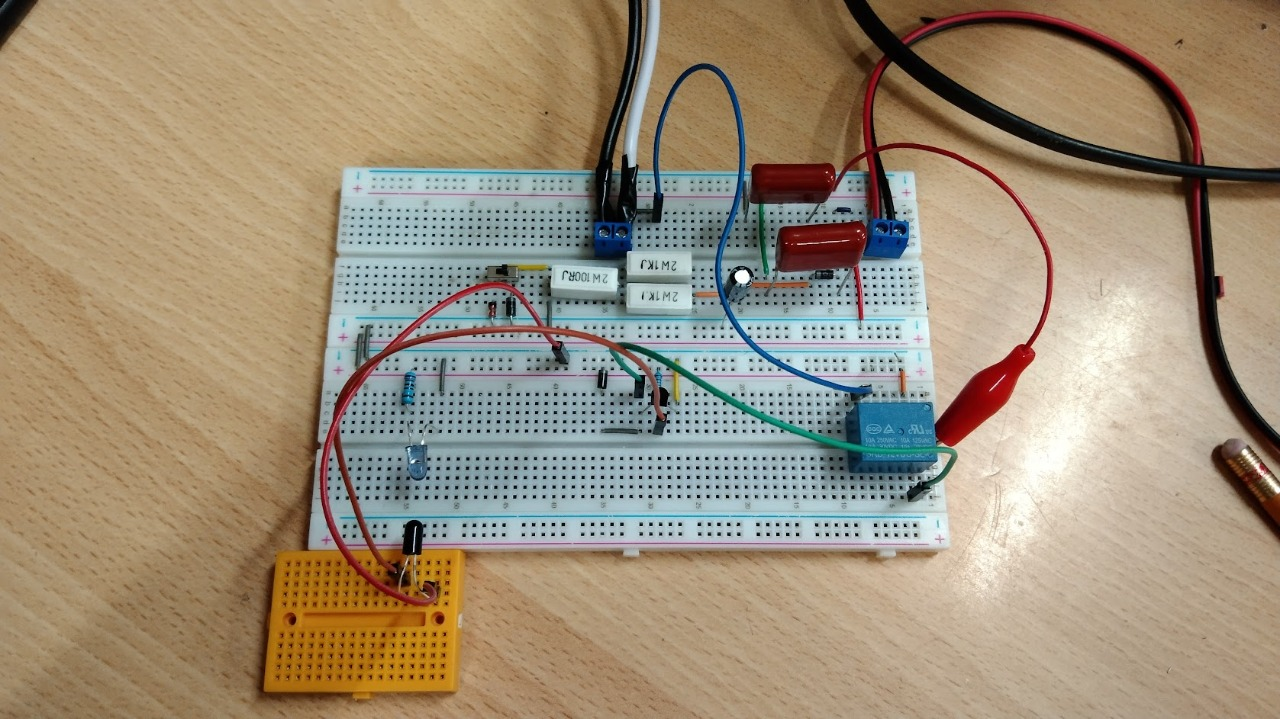
\includegraphics[width=8cm]{media/Practica4.jpg}
    \caption{Armado del circuito con la fuente transformerless}
\end{figure}

\subsection{Resultados}

El circuito funcionó sin ningun problema y con los resultados esperados, en un principio estaba invertido el switch del relé, pero al realizar nuevamente las conexiones, nos
percatamos que el relé estaba mal conectado. De igual manera, la conexión del fototransistor es muy inestable por lo que pudimos apreciar, ya que tuvimos que reconectarlo multiples veces
para identificar que este dispositivo era el que se desactivaba aun conectado, generando confusión en el equipo.

\subsection{Conclusiones}

Esta práctica nos sorprendió en multiples maneras, ya que una de las sorpresas fue la de la fuente sin transformador, la cual no teniamos noción de existencia de ésta,
por lo que pudimos aprender y desarrollar como realizar una opción más de fuente de alimenatción que regula 12V o 5V, según se prefiera.

De igual manera, se apreció que la conexión emisor/receptor por medio de infrarrojo depende de muchos factores, y resulta muy laboriosa y problemática su conexión.
